
\section{Evolving vs dissolving}\label{sec:dissolving}

It is notable that all of the materials that do not show an isotope effect in Table \ref{tab:lattice_lit}, with the possible exception of Pt sputtered on a Teflon DEMS membrane\cite{Willsau1985}, are compact and crystalline films or nanoparticles\cite{Stoerzinger2017, Roy2018, Geiger2018}. In contrast, most of the materials for which studies have seen evidence of lattice oxygen evolution are hydrous, porous, or high-surface-area materials \cite{Wohlfahrt-Mehrens1987, Fierro2007, Surendranath2010, Amin2017, Grimaud2017, Geiger2018}. The authors of these studies all concluded that lattice oxygen is involved in the oxygen evolution mechanism. Equivalently, this implies that an oxygen vacancy is present at some point the electrocatalytic cycle, like in the Mars van Krevelen mechanism from thermal catalysis. However, the observation of an isotope effect does not in itself prove that lattice oxygen evolution is part of a catalytic mechanism. It could, for example, merely part of a parasitic degradation side-reaction. Likewise, many of the studies are not quantitative, and the relative importance of the Mars-van-Krevelin mechanism and other potential OER mechanisms that do not involve lattice oxygen is rarely addressed. 

Lattice oxygen evolution is only compared to dissolution in one of the studies: Geiger et al, 2018, ref. \cite{Geiger2018}. In that study, the authors found that hydrous \ch{Ir^{18}O_x} formed by potential cycling of a sputtered \ch{Ir^{18}O2} film in \ch{^{18}O}-labeled electrolyte, showed lattice oxygen evolution but also increased iridium dissolution compared to the as-sputtered \ch{Ir^{18}O2} film. The authors did not detect lattice oxygen evolution from the as-sputtered film. This comparison of lattice oxygen evolution to dissolution is highly valuable, but the authors did not absolutely quantify the lattice oxygen evolution for direct comparison to dissolution. Particularly, the question I became interested in was: 

\begin{question}
How does the number of lattice oxygen atoms evolved ($n_{\ch{O}}$) compare to the number of metal atoms dissolved ($n_{\ch{M}}$)?\label{q:O_vs_M}
\end{question}

Only if $n_{\ch{O}}\gg  n_{\ch{M}}$, can it be concluded that there is a catalytic mechanism contributing to oxygen evolution which involves lattice oxygen exchange - though this mechanism may still be such a minor portion of the overall oxygen evolution activity as to be of no practical importance. On the other hand, if $n_{\ch{O}}\le  n_{\ch{M}}$, then lattice oxygen evolution might just be part of an unwanted dissolution reaction.

To answer this question, I performed lattice oxygen evolution experiments of the type described in the latter half of the previous Section (Subsections \ref{subsec:Ru_exchange} and \ref{subsec:extraction}), but also collected the electrolyte periodically during the experiment for quantification of metal dissolution with ICP-MS. The procedure for collecting electrolyte during the experiment without losing electrochemical control is described in Subsection \ref{subsec:other_tools}.

I performed these isotope-labeling ``exchange vs dissolution'' experiments on sputtered \ch{Ru^{18}O2} and \ch{Ir^{18}O2} films, electrochemically labeled \ch{Ru} and \ch{Ir} films, and Ru foam. The results are described in the following Subsections.

\subsection{Sputtered \ch{Ru^{18}O2} and\ch{Ir^{18}O2} films}


\begin{figure}[h!]
	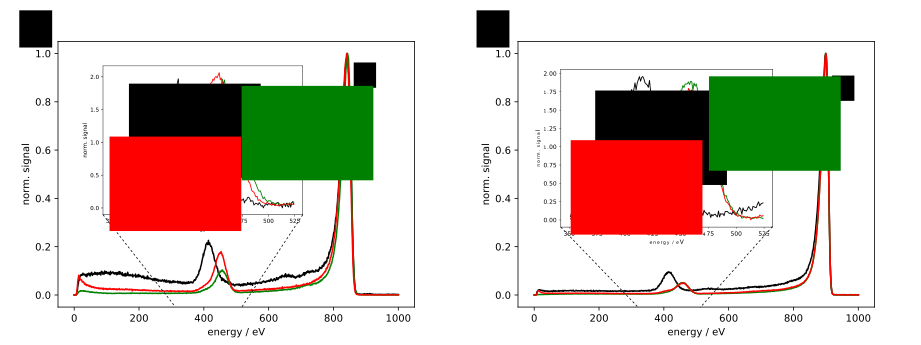
\includegraphics[width=1\textwidth]{04_Oxygen/fig/all_ISS_annotated.png}
	\caption{Ion-scattering spectrometry for isotope-labeled \textbf{(a)} \ch{RuO2} and \textbf{(b)} \ch{IrO2} sputtered films before (green) and after (red) 30 minutes of oxygen evolution at 0.5 mA cm$^{-2}$ in non-labeled electrolyte. Non-labeled films are included for reference (black). The spectra are normalized to the height of the metal peak. The insets show a zoom-in of the oxygen region and are normalized to the combined area of the oxygen peak(s).}
	\label{fig:ISS}
\end{figure}

Of the three strategies for oxygen labeling described in the begining of Section \ref{sec:lattice_O}, strategy C, whereby the as-synthesized catalyst is labeled with \ch{^{18}O}, is preferable whenever possible. It allows for a higher sensitivity than strategy A, in which an un-labeled catalyst is tested in labeled electrolyte, because the labeled electrolyte (typically $\le$ 97\% \ch{^{18}O}) is never as isotopically pure as un-labeled electrolyte (99.8 \% \ch{^{16}O}). On the other hand, it allows for a more well-defined electrocatalytic system than strategy B, in which an un-labeled as-synthesized electrocatalyst is treated electrochemically in labeled electrolyte before testing in un-labeled electrolyte, because the effectiveness of the electrochemical labeling procedure is rarely confirmed and may change the surface of the electrode.

We therefore prepared labeled \ch{Ru^{18}O2} and \ch{Ir^{18}O2} films by reactive sputtering of Ru or Ir with a sputtering plasma consisting of 80\% Ar and 20\% \ch{^{18}O2} (99\% isotopic purity). This produced an isotopically pure as-synthesized electrocatalyst for testing in un-labeled electrolyte.

Labeled oxide films of 25 nm nominal thickness (\ch{Ru^{18}O2}) or 10 nm thickness (\ch{Ir^{18}O2}) were prepared by sputter deposition on glassy carbon substrates with a 5 nm Ti sticking layer. The sputter deposition was done at room temperature, resulting in amorphous \ch{Ru^{18}O2}. The labeling of the as-deposited samples was confirmed by ion scattering spectroscopy as shown in Figure \ref{fig:ISS}. It is notable that the isotopic purity of the oxygen signal in ISS remained high even after the electrode was left out for several days in air, indicating that \ch{RuO2} and \ch{IrO2} do not exchange bound oxygen with the \ch{O2} or \ch{H2O} in air.

\begin{figure}[h!]
	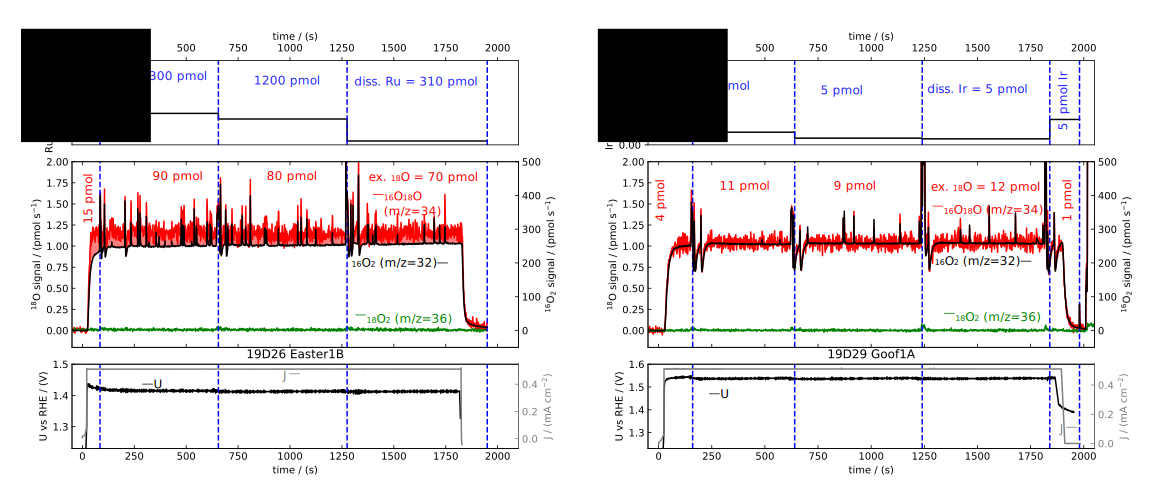
\includegraphics[width=1\textwidth]{04_Oxygen/fig/EC-MS-MS_plots.png}
	\caption{Metal dissolution (top panels) and lattice oxygen evolution (middle panels) from room-temperature sputter-deposited \textbf{(a)} \ch{Ru^{18}O2} and \textbf{(b)} \ch{Ir^{18}O2} films in un-labeled 0.1 M \ch{HClO4}. The \ch{O2} signals are measured \textit{in-situ} and plotted on two axes, scaled according to the natural isotopic ratio to show the excess \ch{^{16}O^{18}O}. The metal dissolution is was measured by determining by ICP-MS the concentration of metal in electrolyte samples taken at intervals indicated by the dotted blue lines.} 
	\label{fig:EC-MS-MS_plots}
\end{figure}

The labeled samples were placed in the chip-based EC-MS setup, oxygen evolution was run for half an hour at 0.5 mA/cm$^2$, and electrolyte samples were taken at intervals (approximately 2 min, 10 min, 20 min, and 30 min) for analysis by ICP-MS. The first ten minutes of electrolysis is shown in Figure \ref{fig:EC-MS-MS_plots}a for the labeled \ch{Ru^{18}O2} film, and in Figure \ref{fig:EC-MS-MS_plots}b for the labeled \ch{Ir^{18}O2} film. The results are plotted as EC-MS-MS plots, with the electrochemistry data in the lower panel, gas flux to the mass spectrometer in the middle panel, and averaged metal dissolution rate in the upper panel, all with a shared time axis. The gas MS data are plotted on two y-axes. The calibrated m/z=34 signal (\ch{^{16}O^{18}O}) is plotted on the right y-axis and the m/z=32 (\ch{^{16}O2}) signal plotted on the left y-axes. The two axes are scaled accordinig to the natural \ch{^{16}O^{18}O}/\ch{^{16}O2} ratio of 0.4\%. Thus, the two traces fall perfectly on top of each other when the oxygen evolved matches the natural isotopic ratio. For the case of \ch{Ru^{18}O2} there is a clear excess of \ch{^{16}O^{18}O} signal compared to the natural ratio. The excess is indicated in the plot with a light red highlight. In the first 10 minutes, there are approximately 100 pmol of lattice \ch{^{18}O} evolved. In comparison, approximately 150 nmol of oxygen was evolved in total. The mechanism by which lattice oxygen is evolved as \ch{O2} thus only accounts for $\approx$0.07\% of the total OER activity during the first ten minutes. For the \ch{Ir^{18}O2} film, the deviation of the \ch{^{16}O^{18}O} signal from the natural ratio is not immediately visible in Figure \ref{fig:EC-MS-MS_plots}, but integration indicates that there is a small excess of $\approx$ 15 pmol of \ch{^{16}O^{18}O} evolved during the first ten minutes, corresponding to less than 0.01\% of the total oxygen evolved. The rate of lattice oxygen evolution decreases only slightly during the remainder of the 30 minutes, such that 250 pmol of lattice oxygen is evolved during 30 minutes for \ch{Ru^{18}O2} and 35 pmol of lattice oxygen is evolved during 30 minutes for \ch{Ir^{18}O2}. In neither case was a significant \ch{^{18}O2} signal observed. 

It should be pointed out that, since the films studied here are isotope-labeled by reactive sputtering in vacuum with isotope-labeled oxygen, they have never been in contact with isotope-labeled water. Thus, incorporated \ch{H2^{18}O} can be ruled out as a source of the excess \ch{^{18}O} evolved, which is more difficult to exclude when films are electrochemically labeled. 

The vertical blue dashed lines indicate when electrolyte samples were taken. There is clear noise in the gas-phase MS data while electrolyte is flowing (middle panel), but with no loss of current control and potential measurement (bottom panel). The amount of metal in the electrolyte sample, in pmol, is indicated before each dotted blue line. This amount, divided by the length of time between electrolyte samples are taken, gives an average dissolution rate in pmol/s. For both the \ch{Ir^{18}O2} and \ch{Ru^{18}O2} samples, the highest dissolution rate was at the start of the electrolysis experiment, as the potential increased from OCP to the operating potential giving 0.5 mA/cm$^2$. In the case of \ch{Ru^{18}O2}, the average dissolution rate remained high, approximately 2 pmol/s, corresponding to a stability number on the order of 100. The amount of ruthenium dissolving into solution was approximately 10 times the amount of lattice \ch{^{18}O} evolved as \ch{^{16}O^{18}O}. For \ch{Ir^{18}O2}, on the other hand, the dissolution quickly lowers to a much smaller rate of ca 90 fmol/s, corresponding to a stability number of approximately 3x10$^4$. The amount of lattice oxygen evolved from \ch{Ir^{18}O2} actually exceeds the amount of iridium dissolved between all electrolyte samples excluding the ramp-up and ramp-down periods.

As a side note of potentially high interest: The apparent Ru dissolution rate for the last electrolyte sample (0.4 pmol/s) is much lower than for the previous two electrolyte samples (2 pmol/s). The main experimental difference is that the last electrolyte sample was taken after the applied potential was turned off, while the catalyst was at OCP. Electrolyte is flowing when the electrolyte sample is taken, and still otherwise, so this may be a case of influencing the thing we are trying to measure. This result indicates that it may be the combination of applied potential and electrolyte flow that leads to \ch{RuO2} dissolution. More experiments are needed specifically probing the effect of electrolyte flow on ruthenium stable. If this is the case that ruthenium is many times more stable in still electrolyte than flowing electrolyte, it could have profound implications for PEM electrolyzers. Such a difference in stability could arise from a small concentration of dissolved ruthenium building up in the electrolyte when it is not flowing. This might imply that PEM electrolyzers with \ch{RuO2} designed to have a small anolyte volume with some concentration of dissolved ruthenium could stabilize ruthenium anodes. This would be revolutionary, as \ch{RuO2} requires less overpotential than the \ch{IrO2} catalyst currently used, and is (slightly) less scarce and thus more scalable. More experiments are needed.

Based on capacitance measurements, a monolayer of the labeled films corresponds to approximately 9 nmol of oxygen for \ch{RuO2} (roughness factor $\approx$ 50) and 3 nmol for \ch{IrO2} (roughness factor $\approx$ 25). The amount of lattice oxygen evolved in the full 30 minutes is thus $\approx$ 3\% of a monolayer for \ch{Ru^{18}O2} and $\approx$ 1\% of a monolayer for \ch{Ir^{18}O2}.

\begin{figure}[h!]
	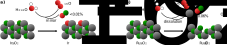
\includegraphics[width=1\textwidth]{04_Oxygen/fig/diagram_lattice_O_evolution.png}
	\caption{Lattice oxygen can either be due to (a) a Mars - van Krevelen type mechanism, as in the case of \ch{IrO2}, or (b) a dissolution side-reaction, as in the case of \ch{RuO2}.}
	\label{fig:exchange_diagram}
\end{figure}

If the lattice oxygen evolution is due to a Mars-van Krevelen type mechanism, then the oxygen isotope present in the electrolyte should be incorporated into the lattice, and should be present in the catalyst after the reaction. If, however, the lattice oxygen evolution is a side-product of a dissolution mechanism, then oxygen from the electrolyte would not be incorporated in the lattice. This is illustrated in Figure \ref{fig:exchange_diagram}. Ion-scattering spectrometry after OER can thus help distinguish between the possibilites. The red traces in Figure \ref{fig:ISS} indicate that little to no \ch{^{16}O} has been incorporated into the surface of the \ch{Ru^{18}O2} sample, whereas a small amount of \ch{^{16}O} has been incorporated into the surface of the \ch{Ir^{18}O2} electrode. This indicates that the very small amount of lattice oxygen exchange observed in \ch{IrO2} may in fact be due to a Mars - van Krevelen type mechanism, whereas the lattice oxygen evolution observed in \ch{RuO2} may just be part of a dissolution process. As an example of such a dissolution process, the \ch{^{16}O^{18}O} signal observed during OER for \ch{Ru^{18}O} could result from the decomposition in the chip or the vacuum chamber of \ch{RuO4} with at least one of the oxygen atoms from the lattice, as \ch{RuO4(g)} has been observed by mass spectrometry during OER on \ch{RuO2}.\cite{Geiger2018} 

These results from oxygen evolution on isotope-labeled films show that lattice oxygen evolution should not be interpreted as evidence of an important oxygen evolution reaction mechanism involving oxygen vacancies without careful, quantitative studies. Specifically, the activity of the lattice-involving mechanism should be compared quantitatively to the overall OER activity, and to the rate of metal dissolution. 

\subsection{Electrochemically labeled films}

\begin{figure}
	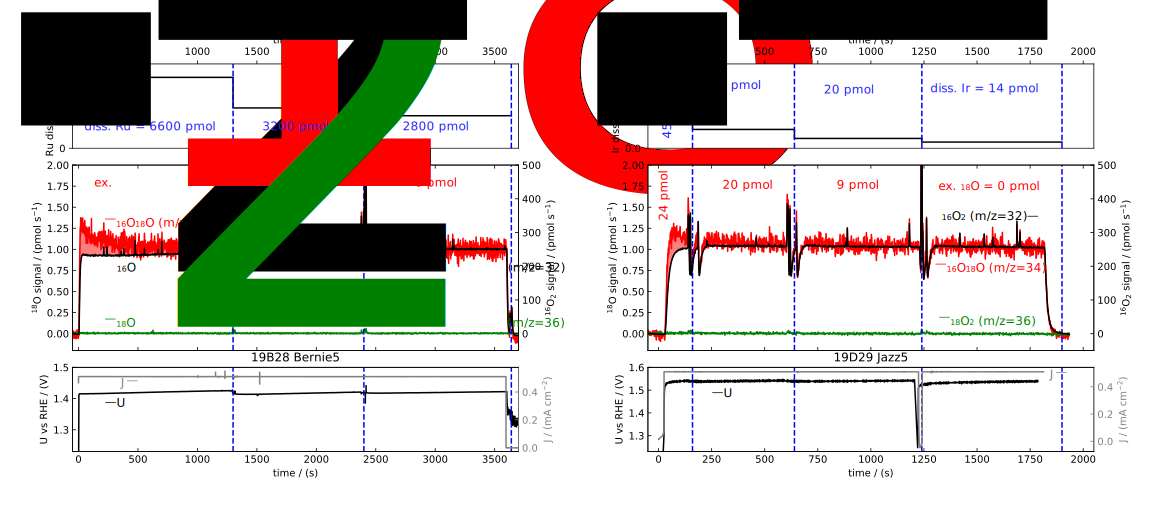
\includegraphics[width=1\textwidth]{04_Oxygen/fig/EC-MS-MS_plots_Electrochemically_labeled.png}
	\caption{Metal dissolution and lattice oxygen evolution from metallic \textbf{(a)} Ru and \textbf{(b)} Ir films in un-labeled 0.1 M \ch{HClO4} after formation electrochemical cycling and oxidation in \ch{^{18}O}-labeled electrolyte.
			}
	\label{fig:EC-MS-MS_EC}
\end{figure}

We also performed the exchange vs dissolution experiments for \ch{Ru} and \ch{Ir} labeled electrochemically. Metallic films of 25 nm thickness (Ru) or 10 nm thickness (Ir) were prepared by sputter deposition on glassy carbon substrates with a 5 nm Ti sticking layer.

The metallic electrodes were placed in the EC-MS setup which was filled with labeled electrolyte (0.1 M \ch{HClO4} in 97\% \ch{H2^{18}O}), where they were first cycled between -0.05 V and +1.4 V (Ru) or +1.5 V (Ir) vs RHE, and then oxidized at +0.5 mA/cm$^2$ geometric current density for 10 minutes. They were then rinsed in natural water and put back in the setup with un-labeled electrolyte (0.1 M \ch{HClO4} in 99.8\% \ch{H2^{16}O}), and subject to a geometric current density of +0.5 mA/cm$^2$ for 30 minutes, with electrolyte taken at intervals for ICP-MS analysis. The results are shown in Figure \ref{fig:EC-MS-MS_EC}.

In both cases, an isotope signal can be seen in the start of the exchange experiment, but in both cases, the integrated excess \ch{^{16}O^{18}O} signal is less than one monolayer equivalent. It is larger for the oxidized \ch{Ru} (Figure \ref{fig:EC-MS-MS_EC}a) than for the oxidized \ch{Ir} (Figure \ref{fig:EC-MS-MS_EC}b). However, in contrast to the sputtered oxide films, in which the isotope signal was more or less steady throughout the 30 minutes of electrolysis, for these electrochemically oxidized films the excess \ch{^{16}O^{18}O} evolution is transient. This could indicate that labeled layer is quite thin and dissolves completely in less than 30 minutes. Indeed, the isotope \ch{^{16}O^{18}O} to \ch{^{16}O2} ratio has converged to the natural isotopic ratio for the oxidized \ch{Ru} film after approximately 9 nmol of \ch{Ru} has dissolved, corresponding roughly to one monolayer. This could indicate that only the outer monolayer had been labeled. Alternately, if the continued oxidation of the metallic film is faster than the dissolution, the labeled oxide layer could be burried beneath an un-labeled oxide layer. This is illustrated in the first panel of Figure \ref{fig:Pt_extraction_diagram}b. This is most likely the reason for the transience of the isotope signal for the iridium electrode, where significantly less than one monolayer of Ir has dissolved before the \ch{^{16}O^{18}O} to \ch{^{16}O2} ratio has converged to the natural isotopic ratio.

In both cases, the amount of metal dissolution is much higher than it is for the sputtered oxide films. This is consistent with prior knowledge that \ch{RuO2} is more stable than \ch{Ru}\cite{Roy2018, Cherevko2016}, and \ch{IrO2} is more stable than \ch{Ir}\cite{Cherevko2016}. 

\begin{figure}
	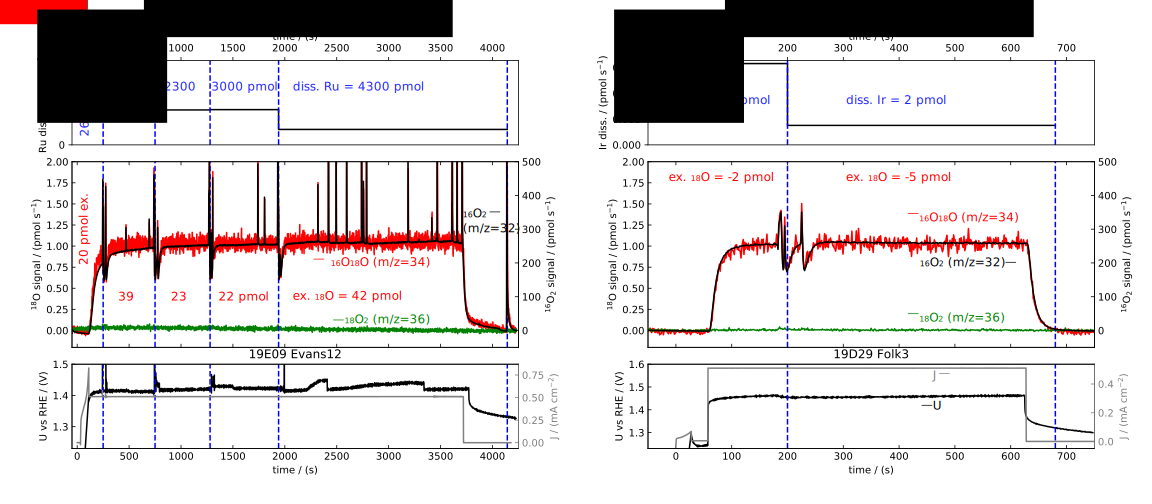
\includegraphics[width=1\textwidth]{04_Oxygen/fig/EC-MS-MS_plot_foam_and_control.png}
	\caption{Metal dissolution and lattice oxygen evolution in un-labeled 0.1 M \ch{HClO4} from \textbf{(a)} Ruthenium foam after oxidation in \ch{^{18}O}-labeled electrolyte, and \textbf{(b)} an un-labeled \ch{Ir^{16}O2} sputtered at 400$^\circ$C as a control.
	}
	\label{fig:EC-MS-MS_foam}
\end{figure}

The same experiment was also performed for a \ch{Ru} foam electrode oxidized at 0.5 mA/cm$^2$ for 30 minutes. The result is shown in Figure \ref{fig:EC-MS-MS_foam}a. Again, the largest rate of excess \ch{^{18}O} evolution is at the beginning. The \ch{^{16}O^{18}O} to \ch{^{16}O2} ratio does not converge completely to the natural isotopic ratio during the 1 hr of measurement, but comes close during the final 30 minutes. This is despite the amount of dissolved ruthenium ($\approx$15 nmol) being much less than a monolayer-equivalent ($\approx$300 nmol) on this high-surface-area film. This film, like that tested in Figure \ref{fig:Evans_extraction} was only oxidized at constant current, and not cycled, in labeled electrolyte. Cycling the electrode in labeled electrolyte leads to a larger amount of labeled oxygen evolution in the exchange experiment (Figure \ref{fig:EC_Ru}). The near-convergence with less than a monolayer of \ch{Ru} dissolved may indicate that the labeled oxide layer becomes buried under an un-labeled oxide layer.

Finally, to validate that the excess \ch{^{18}O} in all of the previous experiments does indeed originate in the electrocatalyst (and not in the vacuum chamber, or an error in the data analysis), we performed a control experiment on an un-labeled \ch{IrO2} film. This film was sputtered on a Ti sticking layer on glassy carbon at 400$^\circ$C in isotopically natural \ch{O2}. The small negative values (-7 pmol total over 10 minutes of electrolysis) obtained when integrating the \ch{^{16}O^{18}O} signal and subtracting that expected based on the \ch{^{16}O2} signal should be taken as an indication of the uncertainty of the method.

\subsection{Exchange and extraction}

Finally, as the last result in this chapter, I show an exchange and extraction experiment (described in Subsection \ref{subsec:extraction}) done with electrolyte sampling for ICP-MS on a sputtered \ch{Ir^{18}O2} film. The entire experiment is shown in Figure \ref{fig:EC-MS-MS_extraction}. Because there's a lot going on, I show the electrochemical program both with the raw \textit{in-situ} MS data (Figure \ref{fig:EC-MS-MS_extraction}a), and again with analyzed \textit{in-situ} MS data and ICP-MS data (Figure \ref{fig:EC-MS-MS_extraction}b). 

\begin{figure}[h!]
	\includegraphics[width=1\textwidth]{04_Oxygen/fig/EC-MS-MS_IrO2_exchange_and_extraction.png}
	\caption{Sequential exchange (OER) and extraction (CO oxidation) experiments on a labeled \ch{Ir^{18}O} film in un-labeled 0.1 M \ch{HClO4}. \textbf{(a)}, raw EC-MS data with all masses plotted on a log scale. The highest mass signal is due to the He (m/z=4) or CO (m/z=28) carrier gas. An air signal is visible whenever electrolyte samples are taken for EC-MS as spikes in m/z=28 (\ch{N2}) and/or m/z=32 (\ch{^{16}O2}) though electrochemically produced \ch{^{16}O2} or \ch{CO} (m/z=28) sometimes interfere with these signals. \textbf{(b)}, Same data, analyzed, with ICP-MS data in the top panel. The labeled signals for \ch{^{16}O^{18}O} and \ch{C^{16}O^{18}O} are plotted on the left y-axis and the un-labeled \ch{^{16}O2} and \ch{C^{16}O2} signals are plotted on the right y-axis. The axes are scaled according to the natural \ch{^{16}O^{18}O} to \ch{^{16}O2} ratio, which is also the natural \ch{C^{16}O^{18}O} to \ch{C^{16}O2} ratio.
	}
	\label{fig:EC-MS-MS_extraction}
\end{figure}

From the left: starting just after t=0, an anodic geometric current density of +0.5 mA/cm$^2$ is applied for 23 minutes. Electrolyte samples are taken after 2 minutes, 10 minutes, and 20 minutes of electrolysis. Each time the electrolyte is exchanged to take a sample for ICP-MS, there is a spike in the m/z=28 signal due to \ch{N2} in the air-saturated electrolyte that is drawn into the cell. Unfortunately, the first electrolyte exchange appears to introduce a bubble, resulting in noise in the m/z=32 (\ch{^{16}O2}) and m/z=34 (\ch{^{16}O^{18}O}) signals starting then and continuing to the end of the electrolysis period. There is also some sporadic noise in the working-electrode potential, which may be because I bumped the alligator clip connecting to the working electrode while exchanging the electrolyte. However, the measured electrode current remains steady at the set value of +0.5 mA/cm$^2$.

Looking at the analyzed data for the same period, the results for lattice oxygen evolution and iridium dissolution are very much as in Figure \ref{fig:EC-MS-MS_plots}b: on the order of 30 pmol of both iridium dissolution and lattice oxygen evolution during the first 20 minutes of electrolysis, but with most of the iridium dissolution coming at the beginning while the potential is changed. Again, during steady electrolysis, the lattice oxygen evolution exceeds the iridium dissolution, indicating that there may be a minor OER mechanism involving lattice oxygen exchange. This confirms that the result is reproducible, and indicates that the method of subtracting the integrated \ch{^{16}O2} signal, weighted by the natural isotopic ratio, from the integrated \ch{^{18}O^{16}O} signal is robust even in the face of noisy data. Again, I emphasize that the lattice oxygen evolution is an extremely small portion - only 0.01\% - of the overall OER activity. 

Continuing towards the right in the raw data: after the electrolysis period, the potential is ramped down to a resting potential of 1.2 V vs RHE (with a small overshoot as I decided on what potential to rest at), and another electolyte sample is taken to see if this small potential ramp resulted in significant \ch{Ir} dissolution (it didn't). Then the carrier gas is changed from He (m/z=4) to CO (m/z=28) to begin the CO oxidation (extraction) portion of the experiment. A very small steady anodic current, on the order of 3 $\mu$A/cm$^2$, is detected right after introduction of \ch{CO}, together with a \ch{C^{16}O2} (m/z=44) signal, and is attributed to steady-state CO oxidation. This steady-state CO oxidation is continued for 15 minutes, during which two electrolyte samples are taken. The electrolyte sampling again brings air-saturated electroyte into the cell. This can no longer be seen in the m/z=28 signal, which is now dominated by CO, but can be seen as an \ch{^{16}O2} (m/z=32) signal. In the analyzed data, it appears that there is a small amount of excess excess \ch{C^{16}O^{18}O} in the \ch{CO2} evolved during this period, but the \ch{C^{16}O^{18}O} (m/z=46) background level is taken when the carrier gas is \ch{He}, and so I can't exclude the possibility that this is because of the effect of \ch{CO} on the background. The iridium dissolution during this period is not significantly above the ICP-MS detection limit of $\approx$ 1 pmol.

The CO oxidation activity at 1.2 V vs RHE is so low because, like \ch{PtO}, \ch{IrO2} is mostly inert for CO oxidation, whereas the metallic surface is active. At about 2500, the potential was scanned slowly (1 mV/s at first, then 5 mV/s) in the cathodic direction. Unlike Pt (Figure \ref{fig:Pt_extraction}), the cathodic scan did not result in a \ch{CO} oxidation transient. Apparently, there is not a sweet spot in between the potential at which an \ch{IrO2} surface is reduced and the potential at which \ch{$*$ OH} can no longer adsorb to oxidize CO by the Langmuir-Hinshelwood mechanism. In the absence of the desired transient, I allowed the cathodic scan to continue all the way down to 0 V vs RHE, where hydrogen evolution occurs, as evidenced by the cathodic current and the m/z=2 signal. This was a mistake, as it likely reduced much of the \ch{^{18}O} out of the surface layer of the electrode, and also dissolved some Ir, as dissolution is known to occur from metal oxide electrodes during the reductive potential sweep\cite{Cherevko2016}. The potential was then scanned anodic again at 5 mV/s, with CO oxidation starting in earnest at about 0.8 V vs RHE. A large transient in the current indicates that an adsorbed monolayer of \ch{CO} was stripped off (CO stripping). Then I went back and forth for a little bit before settling on 0.8 V vs RHE for steady-state extraction. The carrier gas is switched back to He at 3800 s, ending the CO oxidation experiment, and electrolyte is collected at about 4200s for ICP-MS. 

The scans between 2500 and 3200 were not ideal. In an optimal experiment, I would have only scanned the potential to slightly lower than 0.8 V vs RHE, perhaps 0.6 V vs RHE, and then back up, to reduce the surface enough that CO could adsorb, without reducing out lattice \ch{^{18}O}, and then go back up to 0.8 V vs RHE where the CO can be oxidized. Nonetheless, looking at the analyzed data, the procedure had the desired effect. A significant excess of \ch{C^{16}O^{18}O} is produced by CO oxidation, indicating that lattice oxygen can be involved in CO oxidation. 210 pmol of excess \ch{C^{16}O^{18}O} is evolved during CO oxidation, which is significantly more than the excess \ch{^{16}O^{18}O} during OER (40 pmol), and also significantly more than the Ir dissolved during this period (72 pmol) despite the accidental over-reduction of the sample. Because some of the \ch{C^{16}O^{18}O} is expected to lose the \ch{^{18}O} label due to homogeneous exchange with \ch{H2^{16}O} in the electrolyte, the actual amount of lattice O used to oxidize \ch{CO} was more than 210 pmol, though still less than a monolayer equivalent ($\approx$ 3 nmol).

Exchange and dissolution are measured for a second OER period after the CO oxidation experiment. When 0.5 mA/cm$^2$ is applied at 4500s and the potential ramps up to meet this current demand, a \ch{CO2} signal indicates that some \ch{CO} had remained adsorbed on the surface and was oxidized off by the increasing potential. There was a significant excess of \ch{C^{16}O^{18}O} in this \ch{CO2}, indicating that lattice oxygen was involved in stripping off the adsorbed \ch{CO}. There was also much more excess \ch{^{16}O^{18}O} in the \ch{O2} evolved during this second exchange experiment than the first, which may be due to a roughening or destabilizing effect of the potential cycling during the \ch{CO} oxidation portion of the experiment. 

It is worth pointing out that, despite these multiple independent clear observations of lattice oxygen reactivity, all of the lattice \ch{^{18}O}  evolved either in \ch{O2} or \ch{CO2} during the entire exchange + extraction + exchange experiment remained less than one monolayer equivalent.


\subsection{Conclusion and perspective}

If, after reading this Chapter, you get an impression that all of the results remain a bit preliminary, please know that I am right there with you. 

The results presented in this Section, combining isotopic labeling by reactive sputtering with \ch{^{18}O2}, surface isotopic characterization by ISS, fluent electrolyte sampling during the experiments for dissolution measurements by ISS, and routine and confident detection of sub-picomol per second rates of lattice oxygen evolution, all came together during the last months of my PhD. The results presented in the previous Sections and Chapters (as well as Paper \ref{Roy2018}) have indicated some of the trial-and-error, mistakes, and development that was necessary to get there.

The goal is of course to use these tools and techniques to make breakthrough discoveries in OER catalysis that can lead to more efficient and cost-effective PEM electrolyzers. I expect that this could happen by the following paths:

\begin{itemize}
\item Insights based on the newly-detected changes in the Tafel slope of \ch{RuO2} (Section \ref{sec:low_O2}) will help inform theorists about which elementary steps and intermediates are most important in predicting materials that can catalyze the OER at high rates at lower overpotentials.

\item Quantitative comparison of lattice oxygen evolution, total oxygen evolution, and metal dissolution on an atom basis will help make it clear whether ''activating lattice oxygen'' is actually a desired strategy. Based on the results presented here so far on \ch{RuO2} and \ch{IrO2}, it seems that lattice-involving mechanisms are associated with instability and, in any case, only contribute a very small portion of the overall OER activity. Hopefully this will help direct the efforts of the research community.

\item The ease and sensitivity of quantitative OER activity measurements and metal dissolution measurements using the EC-MS setup and ICP-MS of the collected electrolytes will make these techniques a powerful screening tool for acid OER catalysts that are stable and active with less precious metal.
\end{itemize}

Next steps could include applying the techniques presented here to compare activity, exchange, and dissolution on calcined \ch{Ir} and \ch{Ru} containing catalysts more closely resembling the industrially-used ''dimensionally stabilized anodes''\cite{Escudero-Escribano2018}, and promising recently-reported materials based on alloying of Ir and Ru with non-noble metals\cite{Reier2015a, Seitz2016, Diaz-Morales2016a}. An obvious starting point would be to re-visit the thermal-decomposition \ch{IrO_x} result reproduced in Figure \ref{fig:Roy2018_raw_results} from Reference \citen{Fierro2007}, which showed significant lattice oxygen evolution but for which dissolution and ISS were not measured. Some of this work is already being done by Mayrhofer and coworkers \cite{Geiger2018}, but the sensitivity of our EC-MS setup and the combination with ISS can add a lot.

In the next Chapter, the last Chapter of this Thesis, I will attempt to gauge the possible net impact of this work on the climate crisis described in Chapter \ref{ch:Intro}. To do so, I will assume that one or more of the possible impact paths above lead to a reduction of 0.1 mV in the overpotential needed to drive PEM electrolyzer cells, holding all else constant.